\subsection{Тестирование программного средства}

В данном разделе приводится демонстрация работы разработанного программного средства обнаружения аномалий в audit-логах Kubernetes-кластера. Рассматривается полный сценарий взаимодействия пользователя с системой — от настройки источника данных до получения результатов обнаружения аномалий.

Общий процесс работы с приложением включает следующие этапы:

\begin{enumerate}
    \item аутентификация пользователя;
    \item настройка интеграции с источником данных (OpenSearch);
    \item создание модели обнаружения аномалий;
    \item запуск обучения модели;
    \item запуск задачи обнаружения аномалий;
    \item анализ полученных результатов.
\end{enumerate}

Взаимодействие пользователя с системой осуществляется с помощью web-интерфейса, представленного на рисунке~\ref{fig:web_ui}.

\begin{figure}
    \centering
    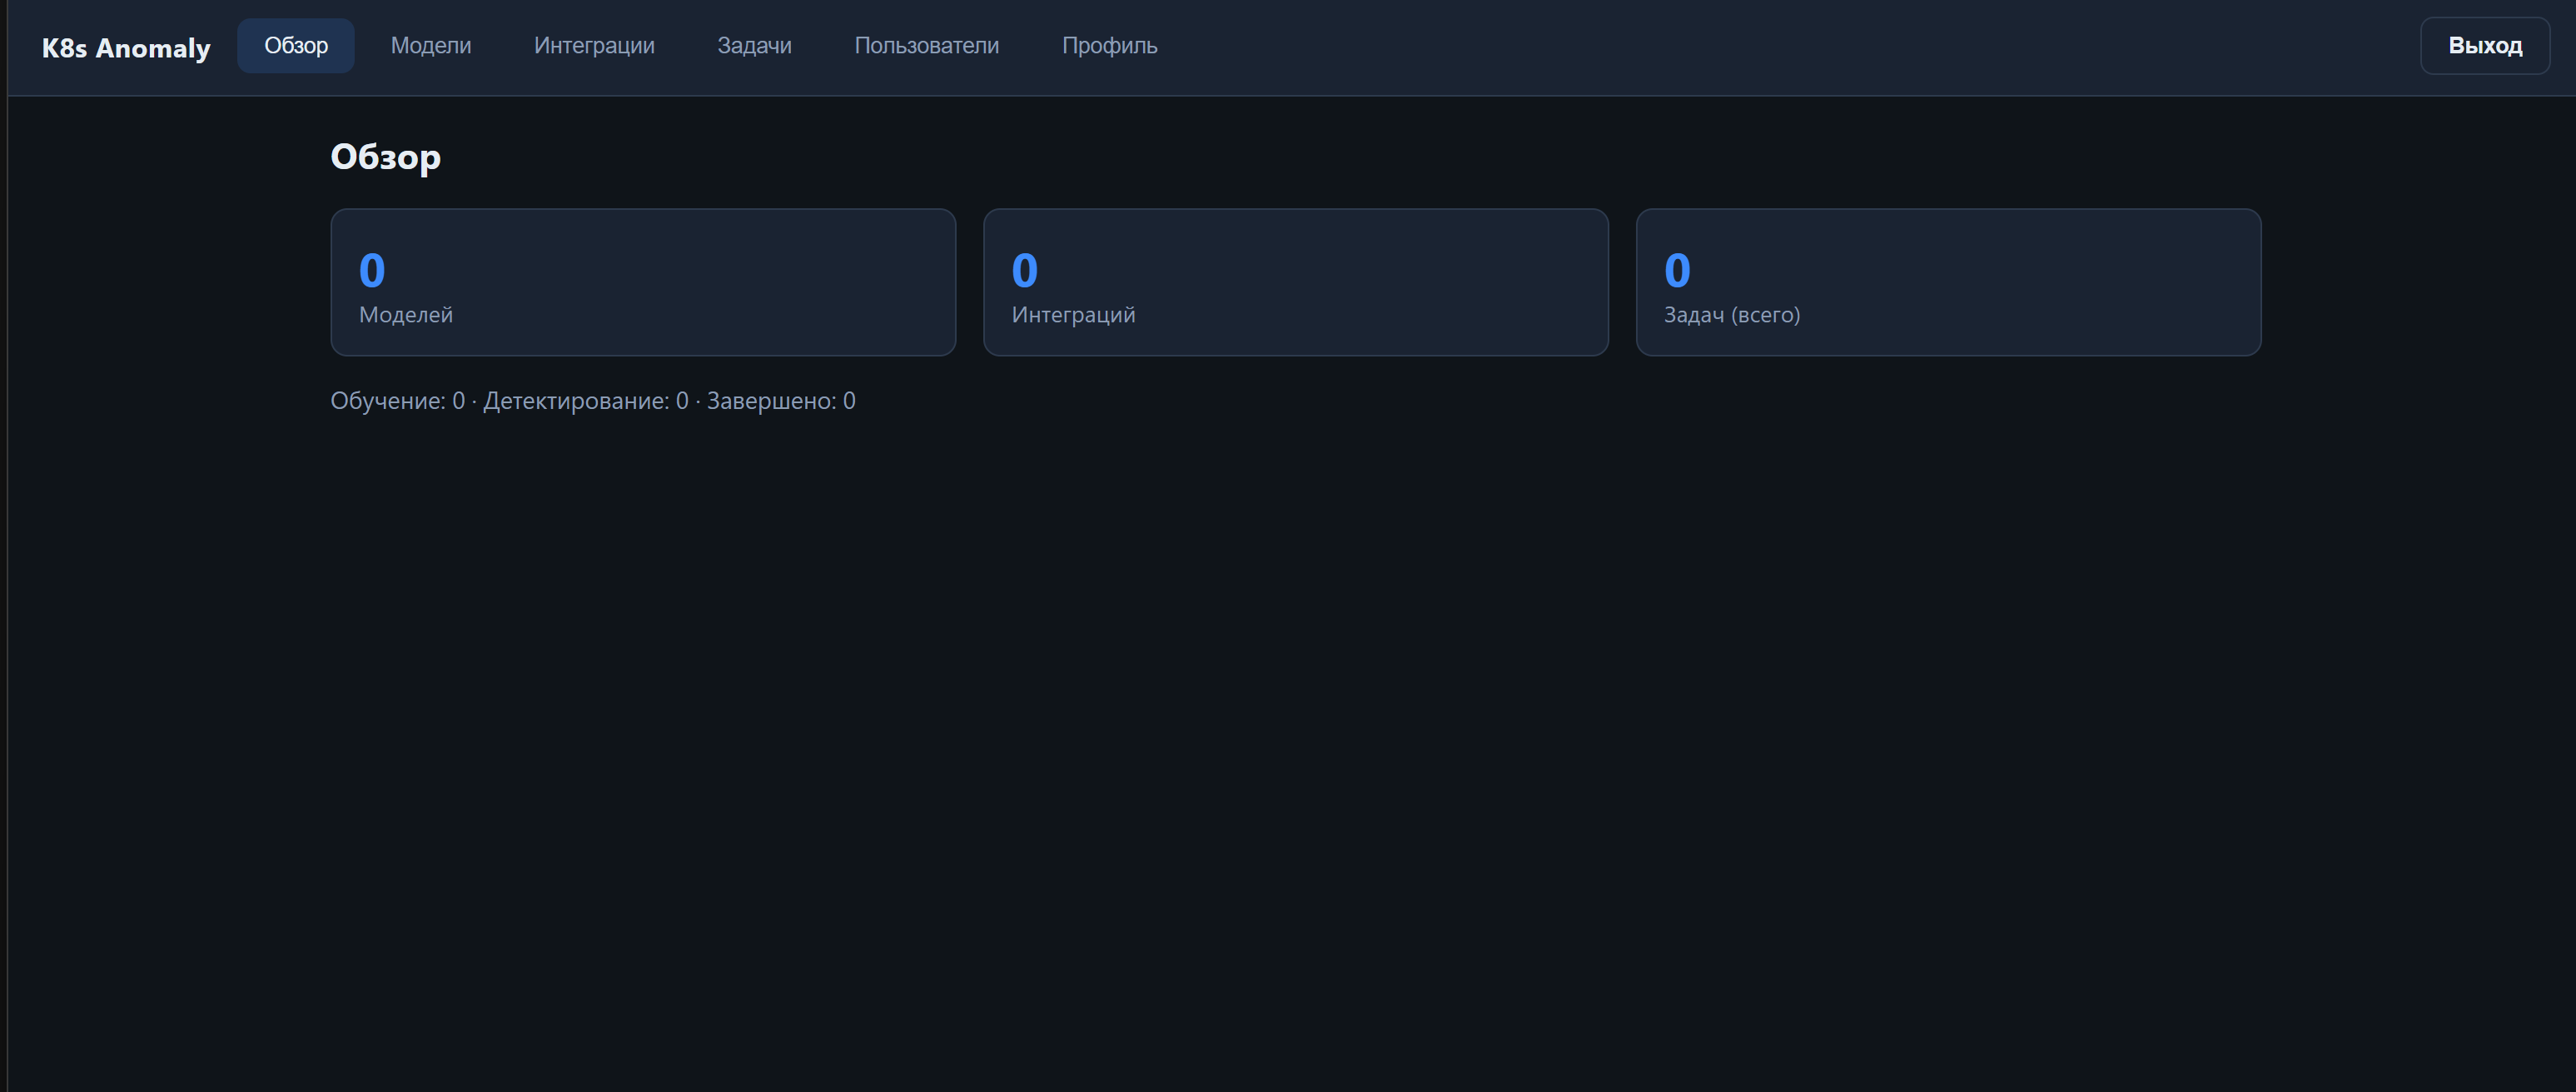
\includegraphics[scale=0.2]{inc/images/web_ui}
    \caption{Интерфейс взаимодействия пользователя}
    \label{fig:web_ui}
\end{figure}

Данный интерфейс позволяет выполнять тестирование всех доступных методов системы, включая создание интеграций, моделей и запуск задач.

На первом этапе пользователь настраивает подключение к источнику audit-логов. Для этого через API передаются параметры подключения к OpenSearch: адрес сервера, учетные данные и имя индекса.

Пример выполнения запроса на создание интеграции представлен на рисунке~\ref{fig:create_integration}.

\begin{figure}
    \centering
    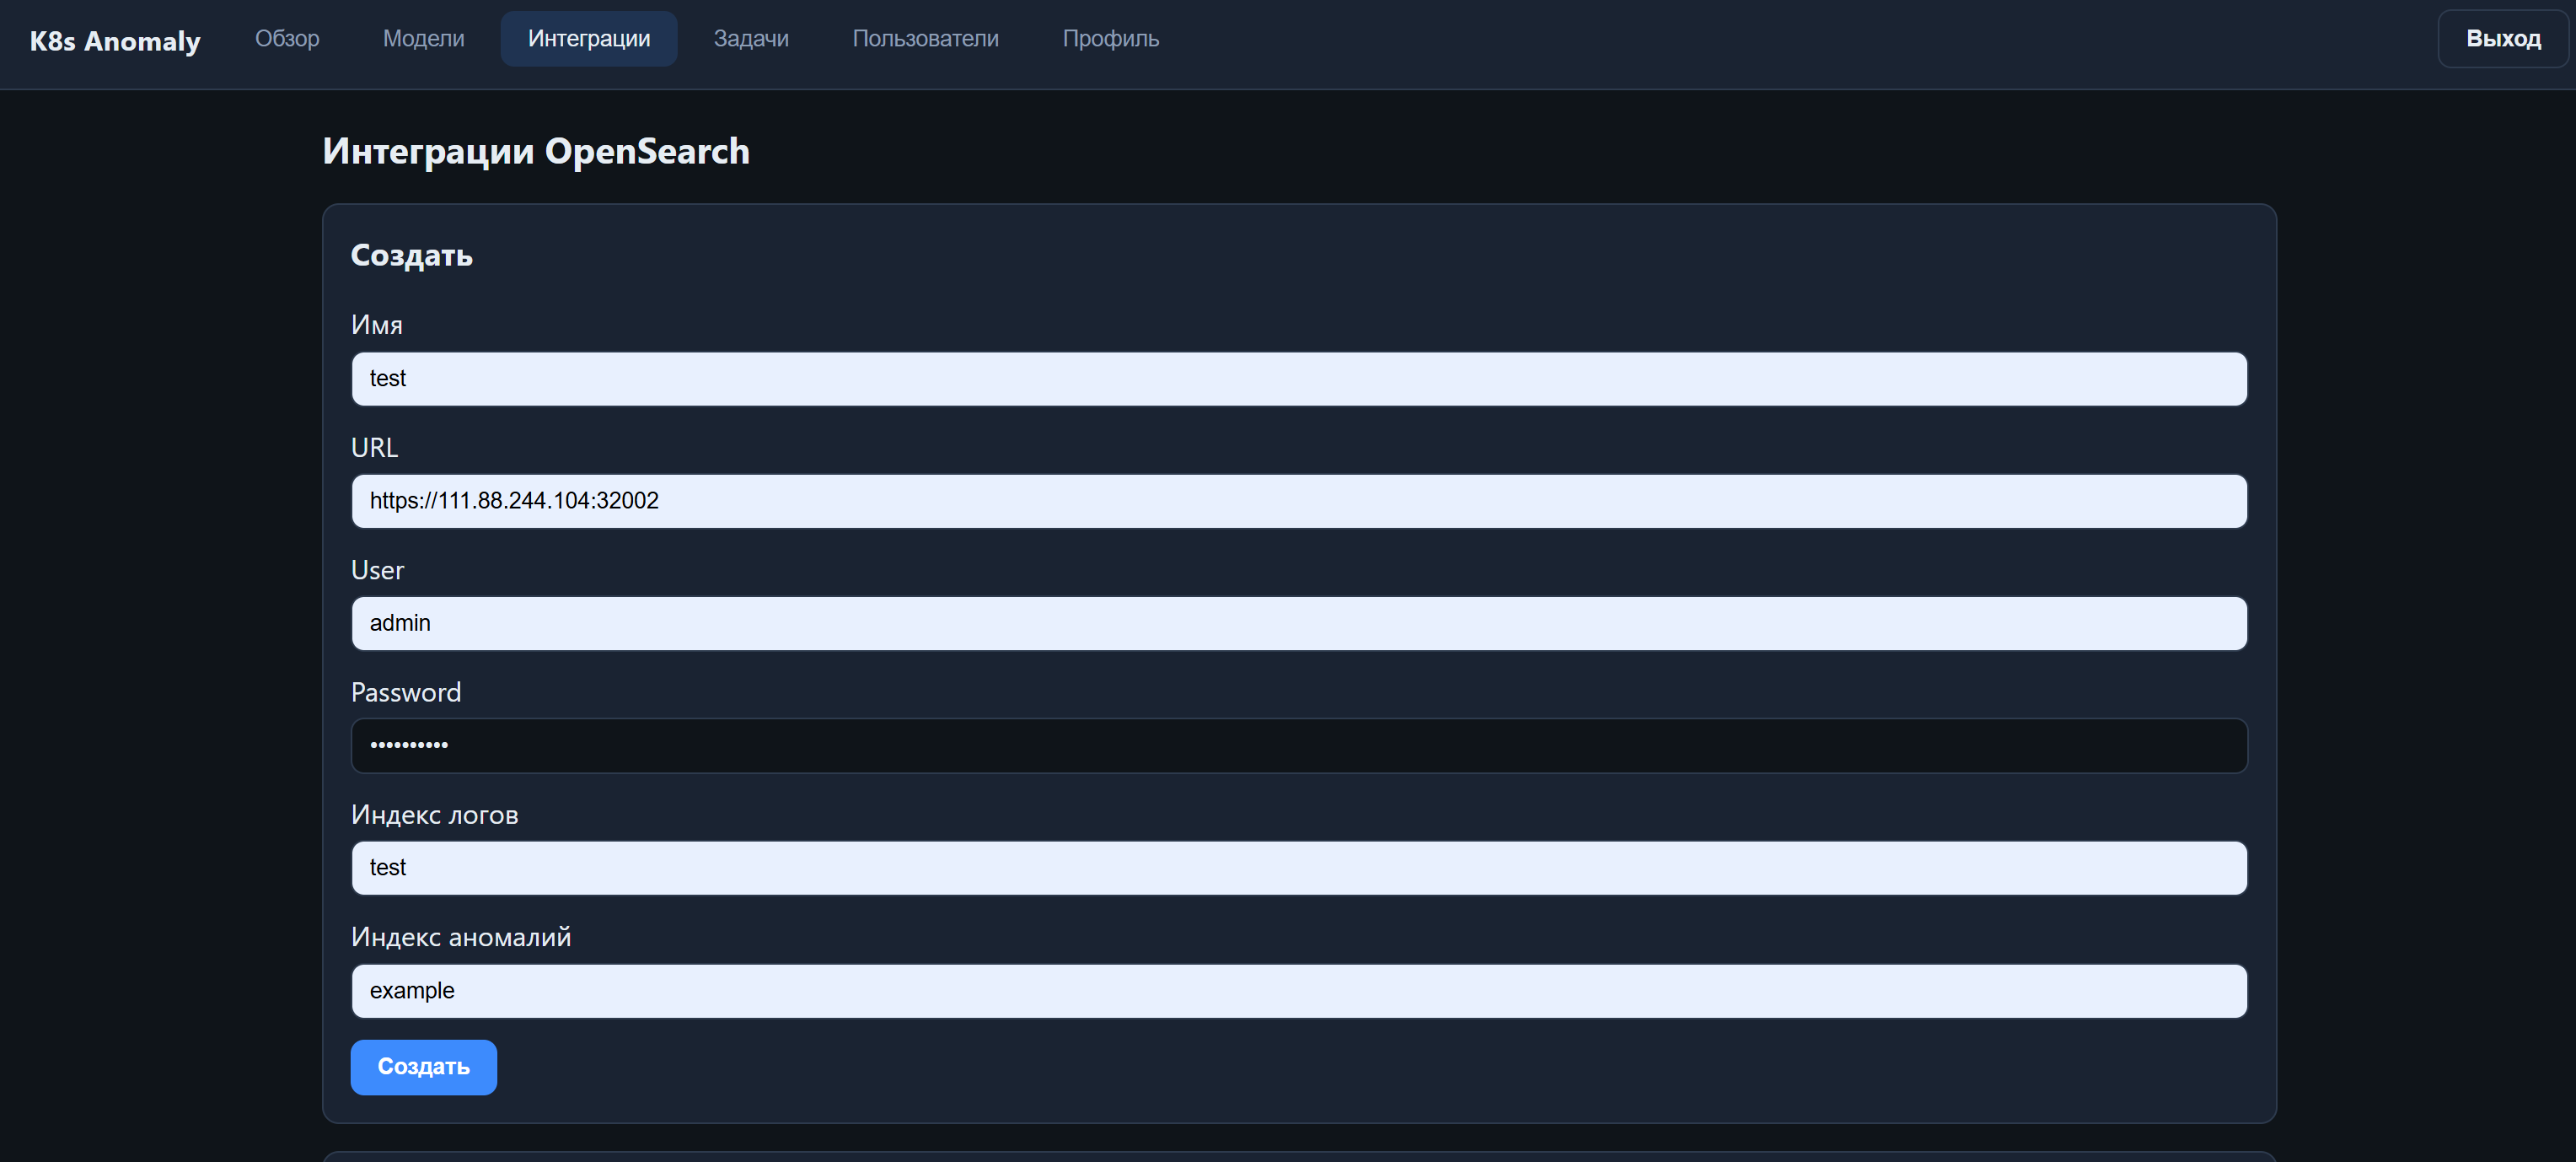
\includegraphics[scale=0.2]{inc/images/create_integration}
    \caption{Создание интеграции с OpenSearch}
    \label{fig:create_integration}
\end{figure}

После отправки запроса система выполняет проверку соединения и сохраняет параметры интеграции в базе данных.

После настройки источника данных пользователь создаёт модель обнаружения аномалий. Пример создания модели представлен на рисунке~\ref{fig:create_model}.

\begin{figure}
    \centering
    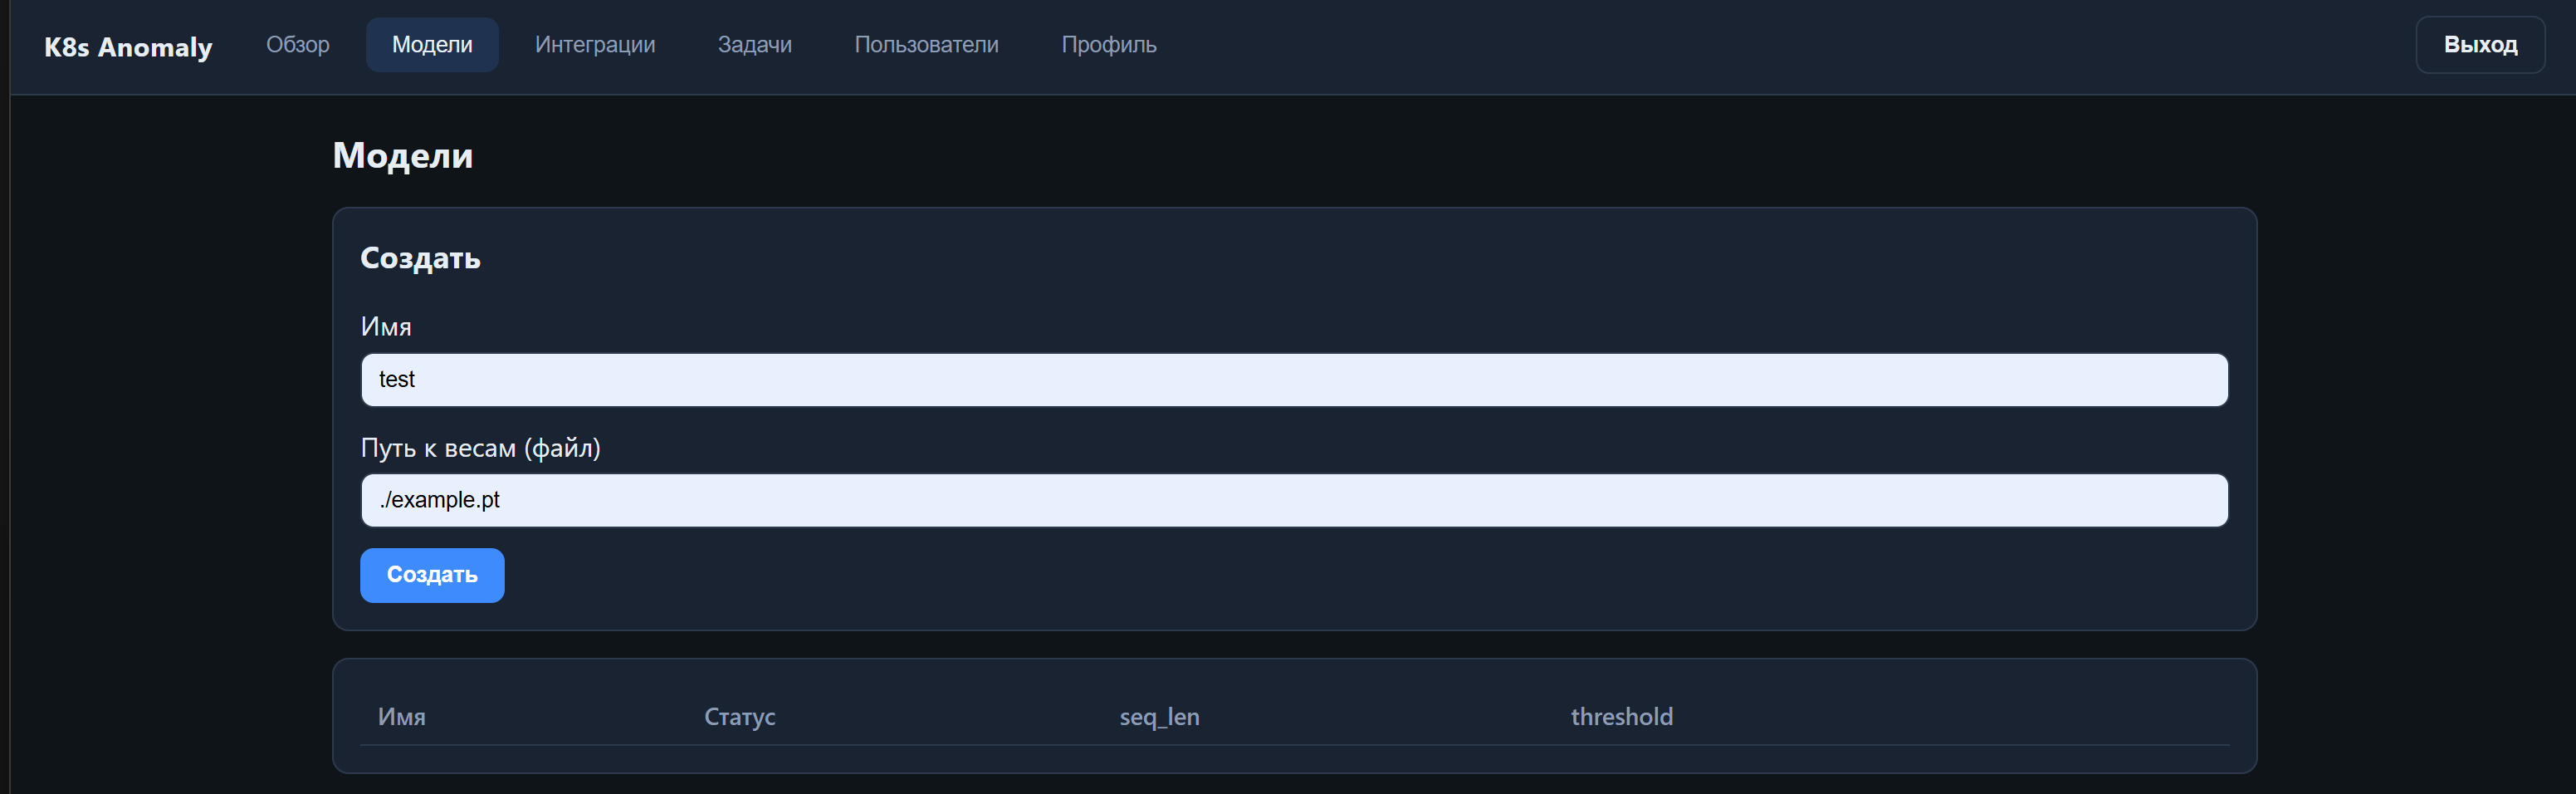
\includegraphics[scale=0.2]{inc/images/create_model}
    \caption{Создание модели обнаружения аномалий}
    \label{fig:create_model}
\end{figure}

После выполнения операции в базе данных создаётся запись о модели со статусом \textit{created}. Обучение модели инициируется пользователем после создания задачи типа \textit{train}, которая помещается в очередь задач. Пример запуска обучения представлен на рисунке~\ref{fig:start_training}.

\begin{figure}
    \centering
    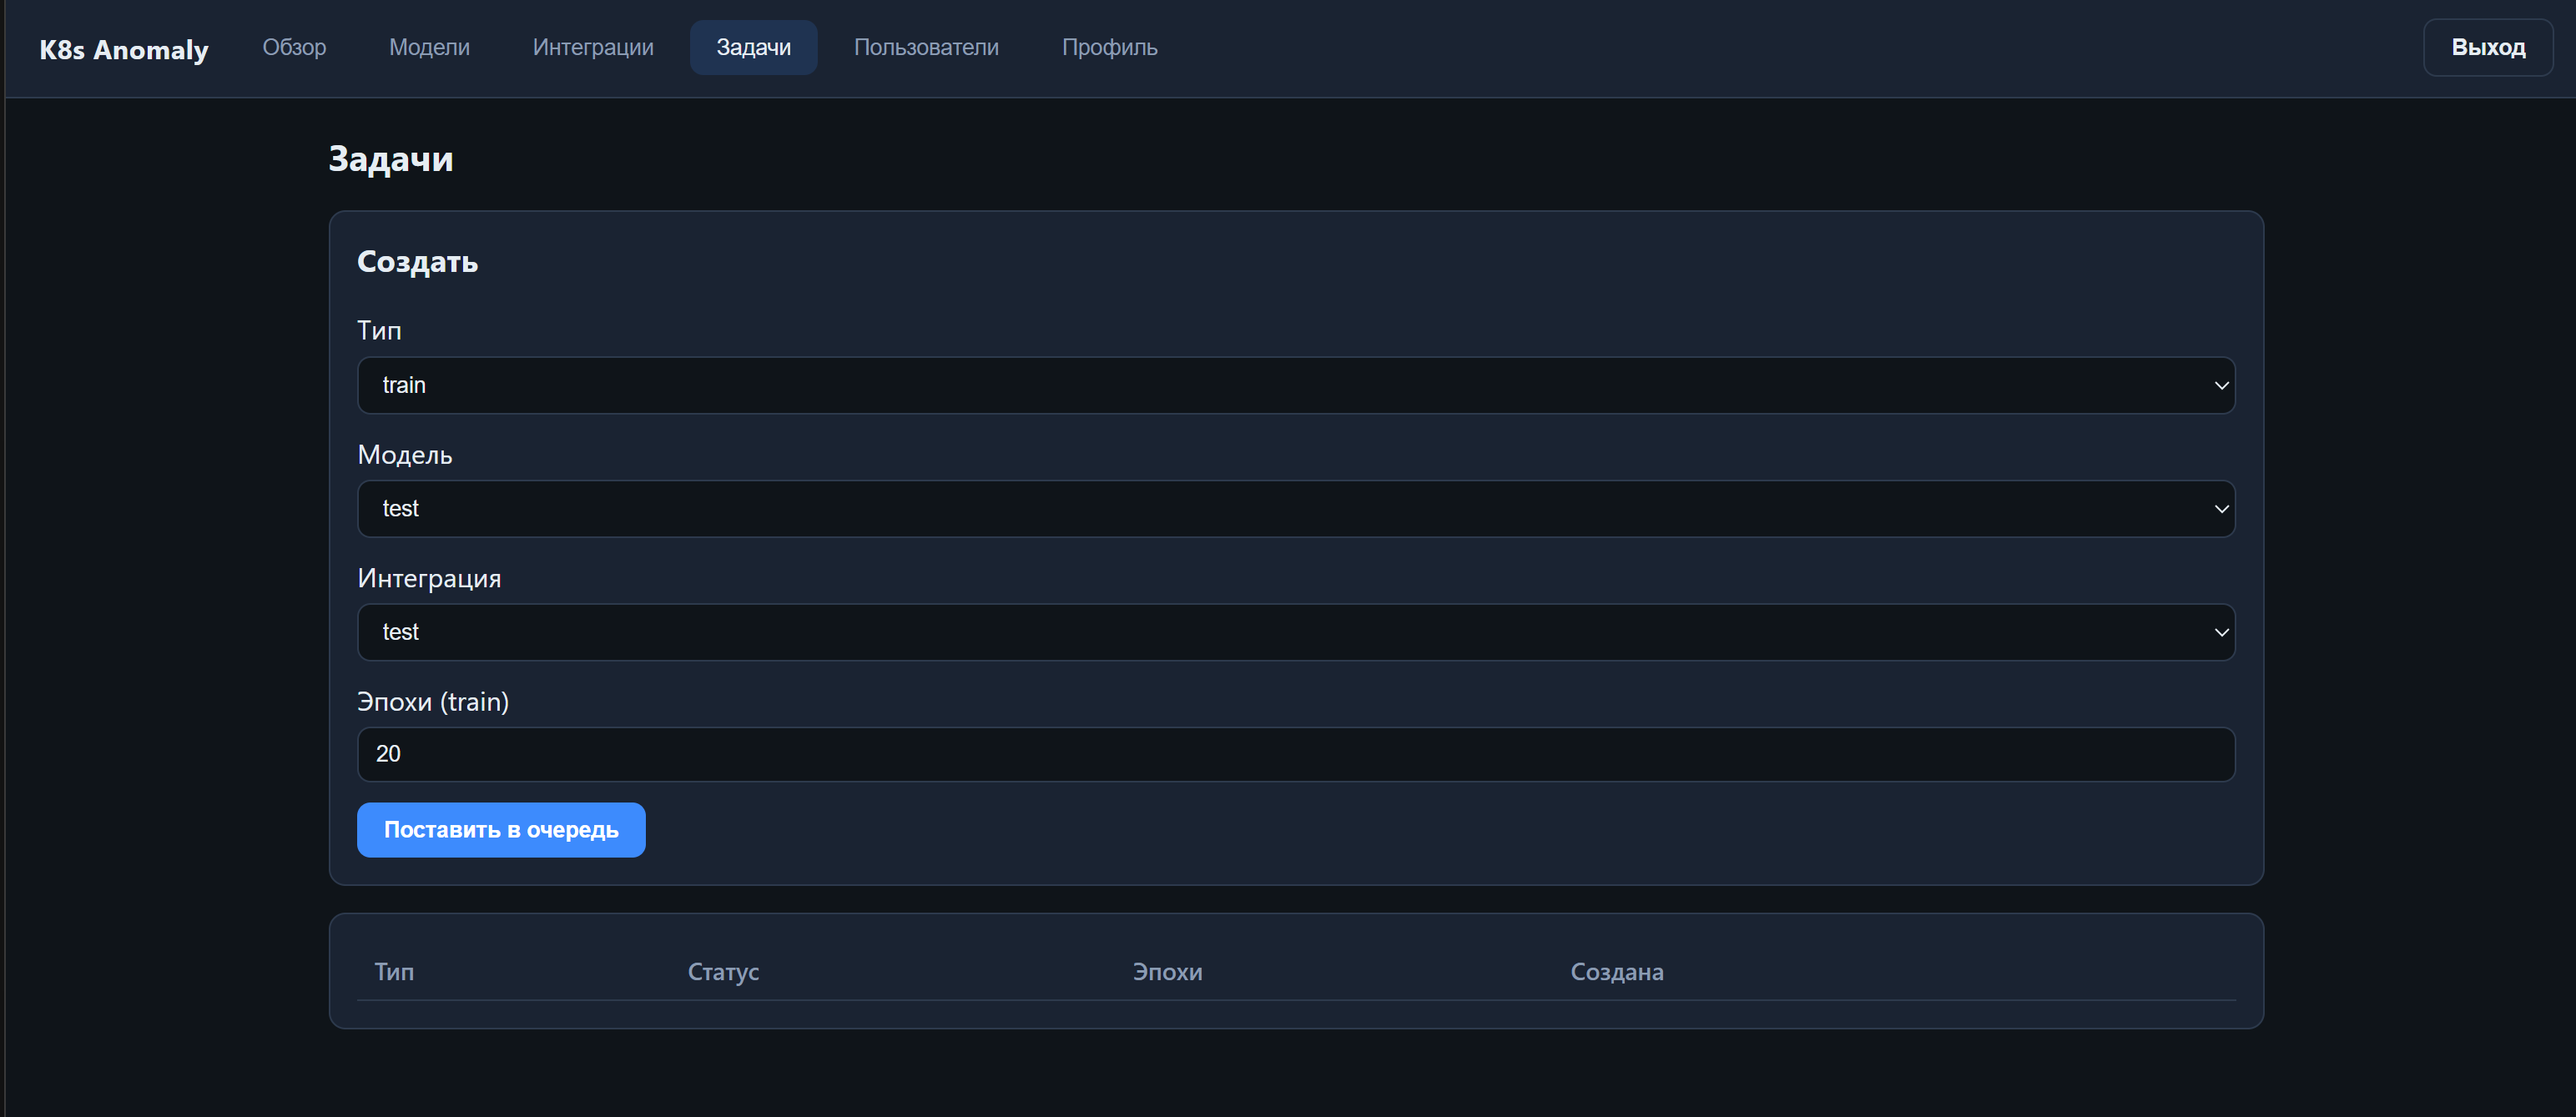
\includegraphics[scale=0.2]{inc/images/start_training}
    \caption{Запуск задачи обучения модели}
    \label{fig:start_training}
\end{figure}

После постановки задачи в очередь она проходит несколько состояний: \textit{starting}, \textit{pending}, \textit{running}, \textit{done}. В процессе обучения вычисляются значения функции потерь, характеризующие качество модели. Пример графика изменения функции потерь приведён на рисунке~\ref{fig:training_loss_demo}.

\begin{figure}
    \centering
    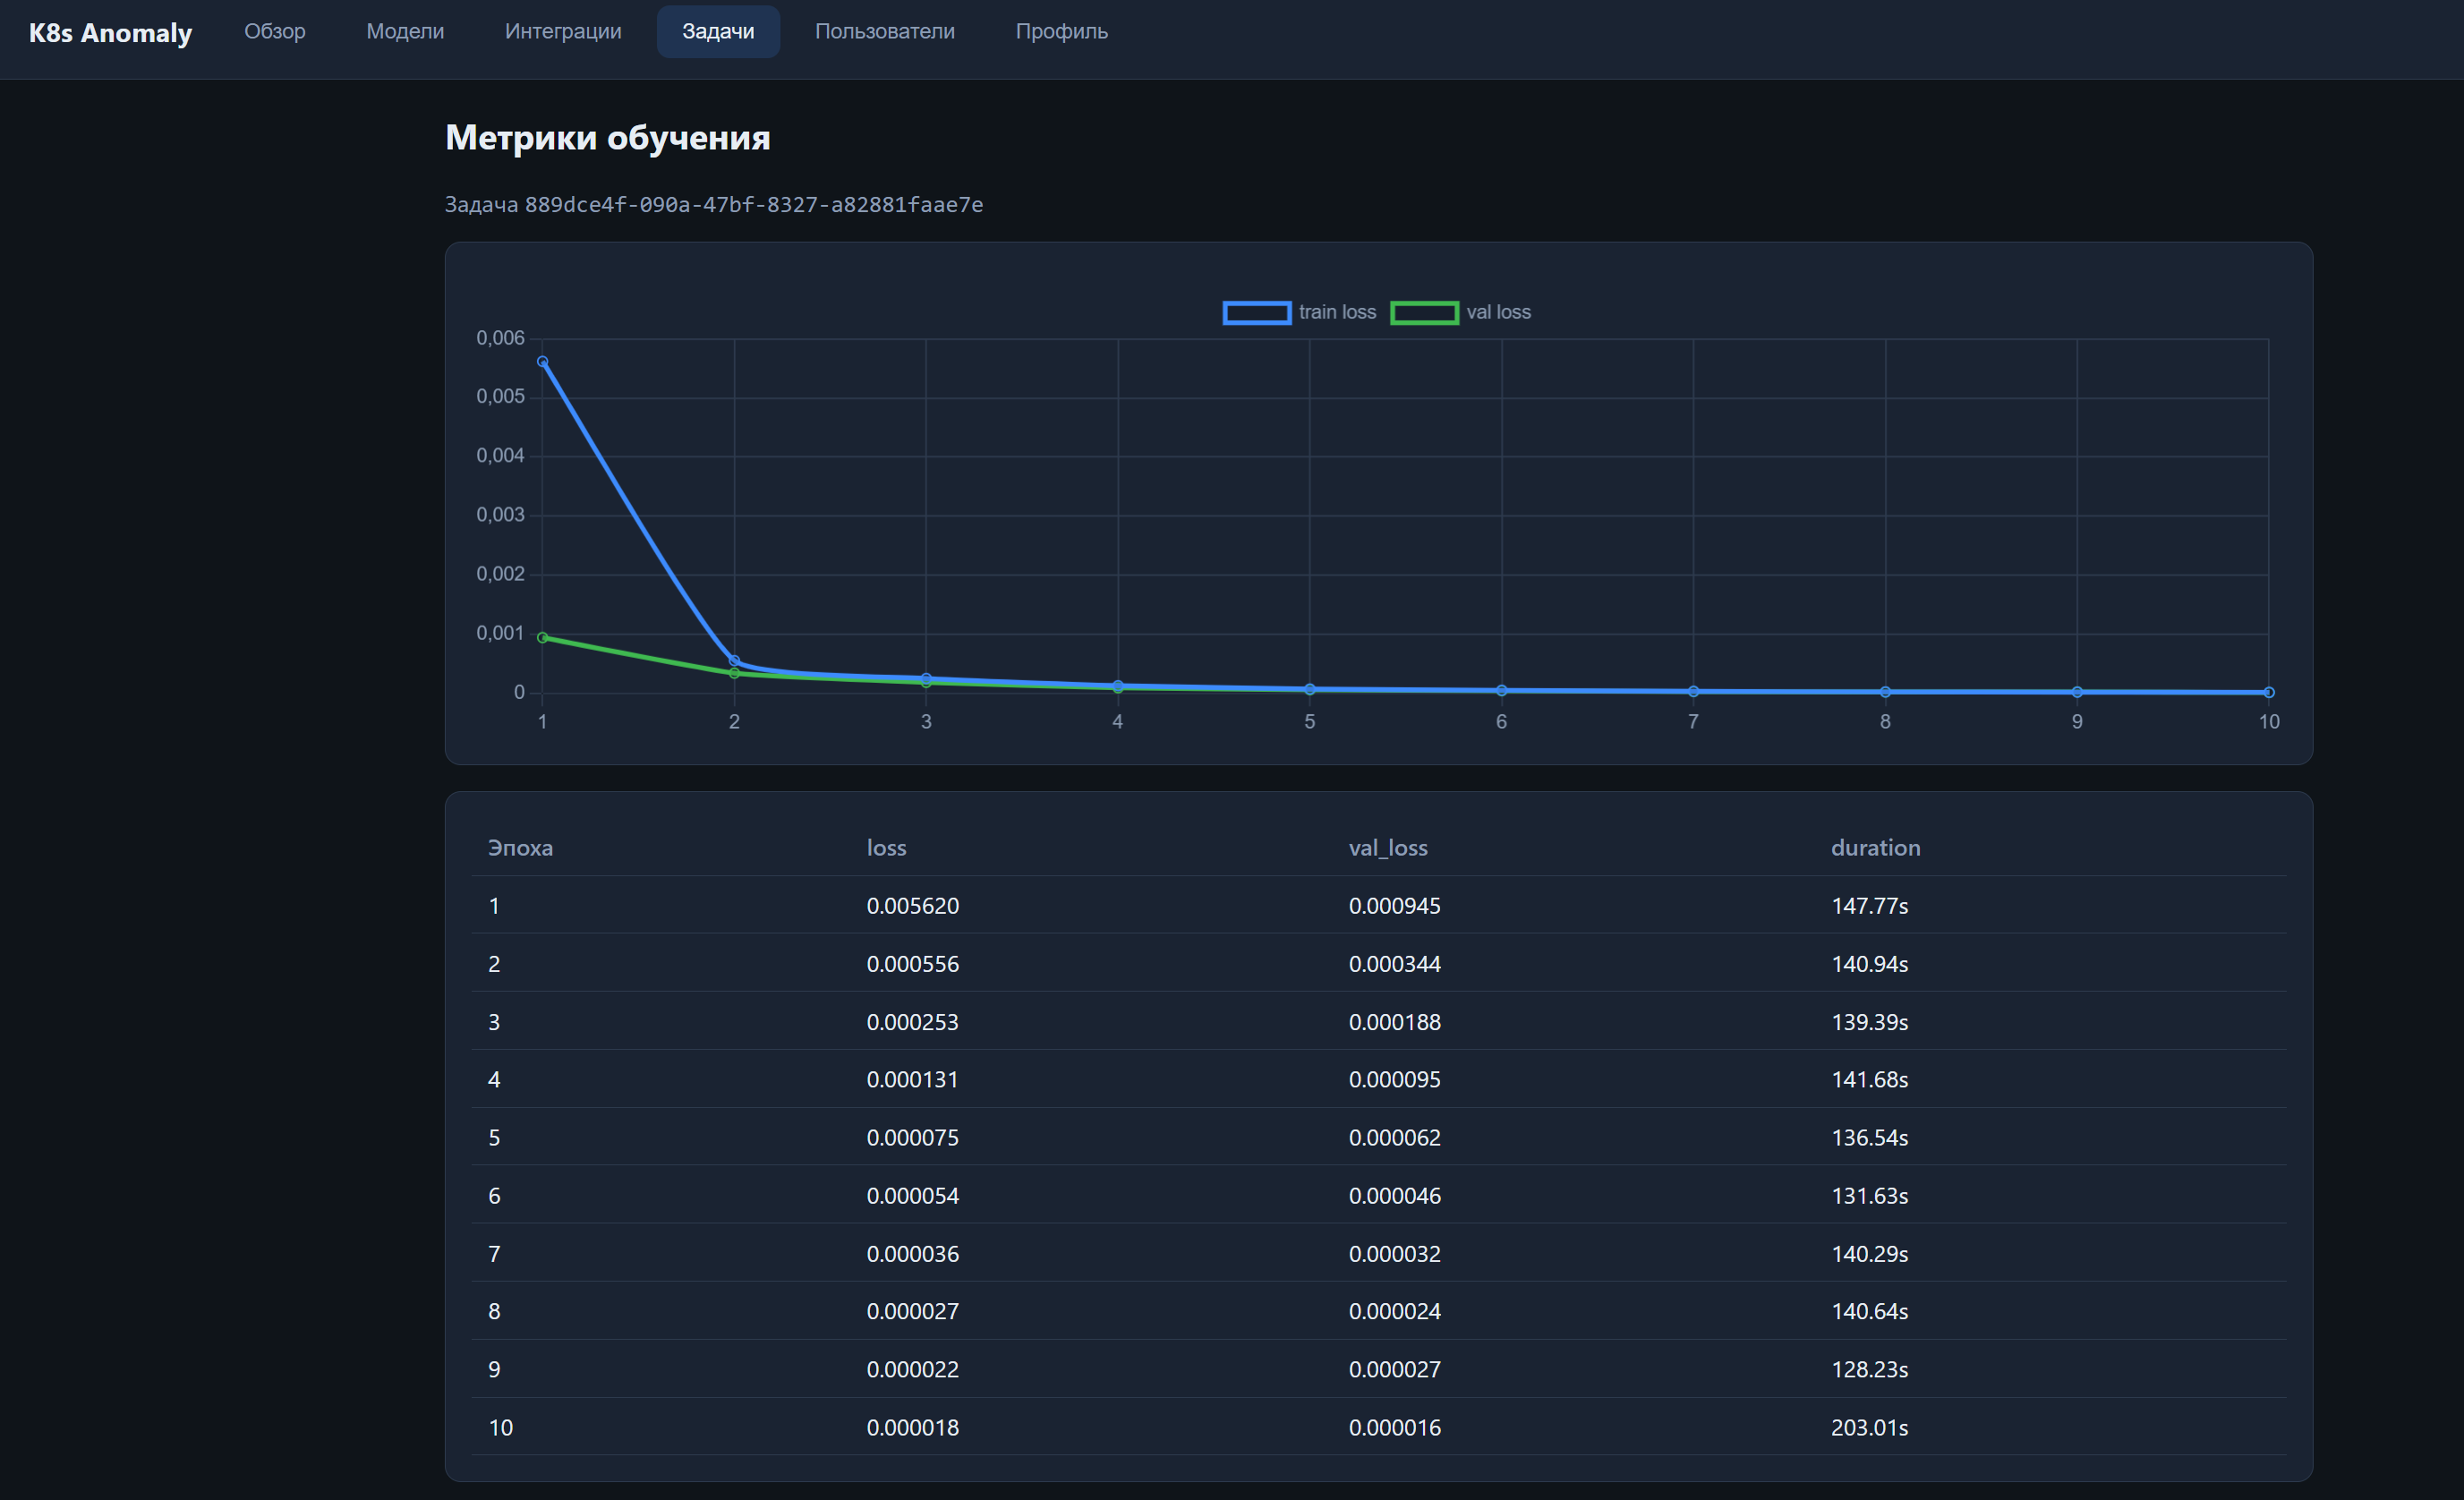
\includegraphics[scale=0.35]{inc/images/training_loss_demo}
    \caption{График функции потерь в процессе обучения модели}
    \label{fig:training_loss_demo}
\end{figure}

После завершения обучения веса модели сохраняются во внешнем хранилище, а сама модель переводится в состояние \textit{ready}.

После обучения модели пользователь может запустить задачу обнаружения аномалий. Процесс аналогичен обучению и также реализуется через очередь задач. Пример запуска задачи детектирования представлен на рисунке~\ref{fig:start_detect}.

\begin{figure}
    \centering
    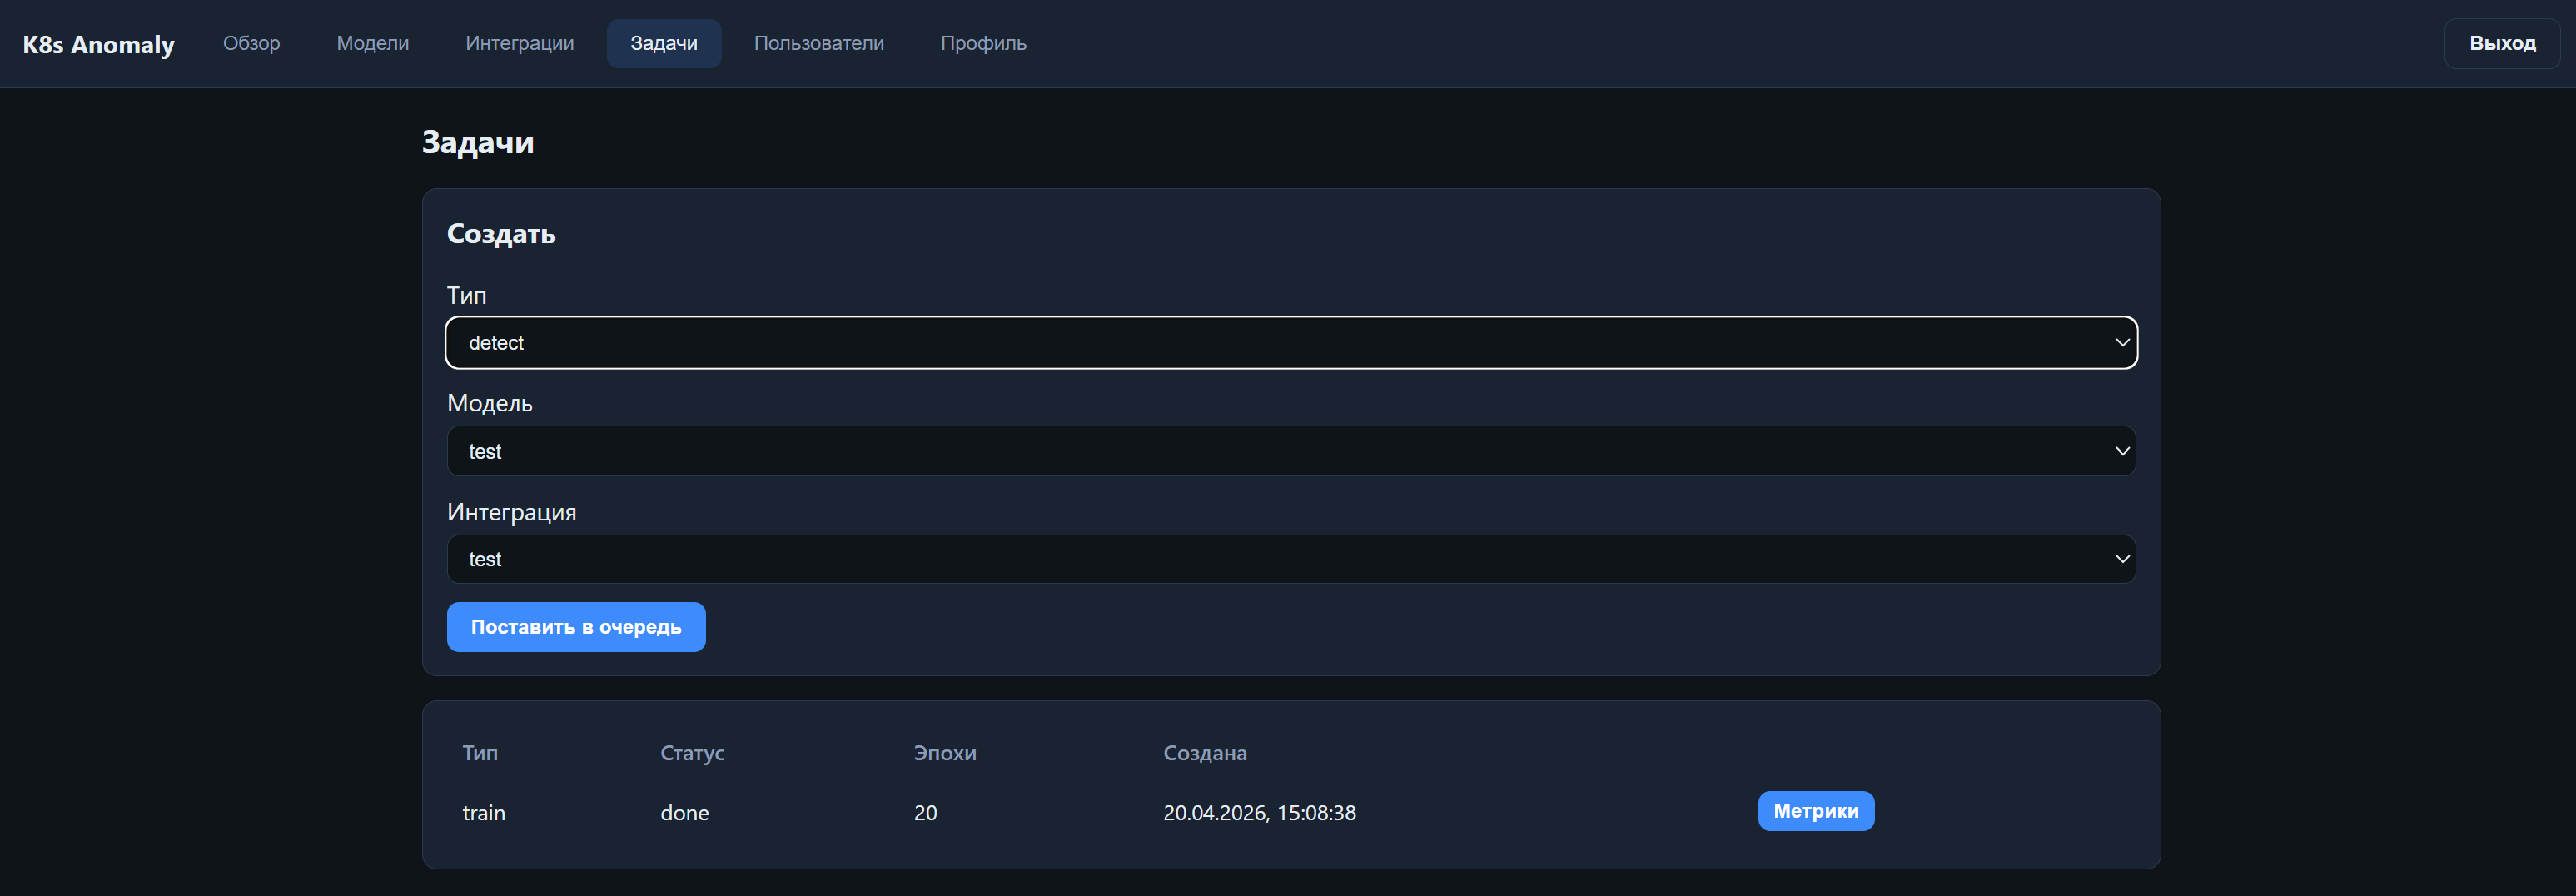
\includegraphics[scale=0.35]{inc/images/start_detect}
    \caption{Запуск задачи обнаружения аномалий}
    \label{fig:start_detect}
\end{figure}

Worker-компонент загружает обученную модель, извлекает данные из OpenSearch и выполняет анализ последовательностей событий.

Результатом работы системы являются выявленные аномальные события, которые сохраняются в отдельном индексе OpenSearch, а также агрегированные метрики, записываемые в базу данных. Система предоставляет пользователю информацию о выполненных задачах, включая:

\begin{itemize}
    \item количество обработанных событий;
    \item число обнаруженных аномалий;
    \item временные характеристики выполнения задачи;
    \item метрики качества модели.
\end{itemize}

Пример отображения результатов выполнения задачи представлен на рисунке~\ref{fig:metrics_example}.

\begin{figure}
    \centering
    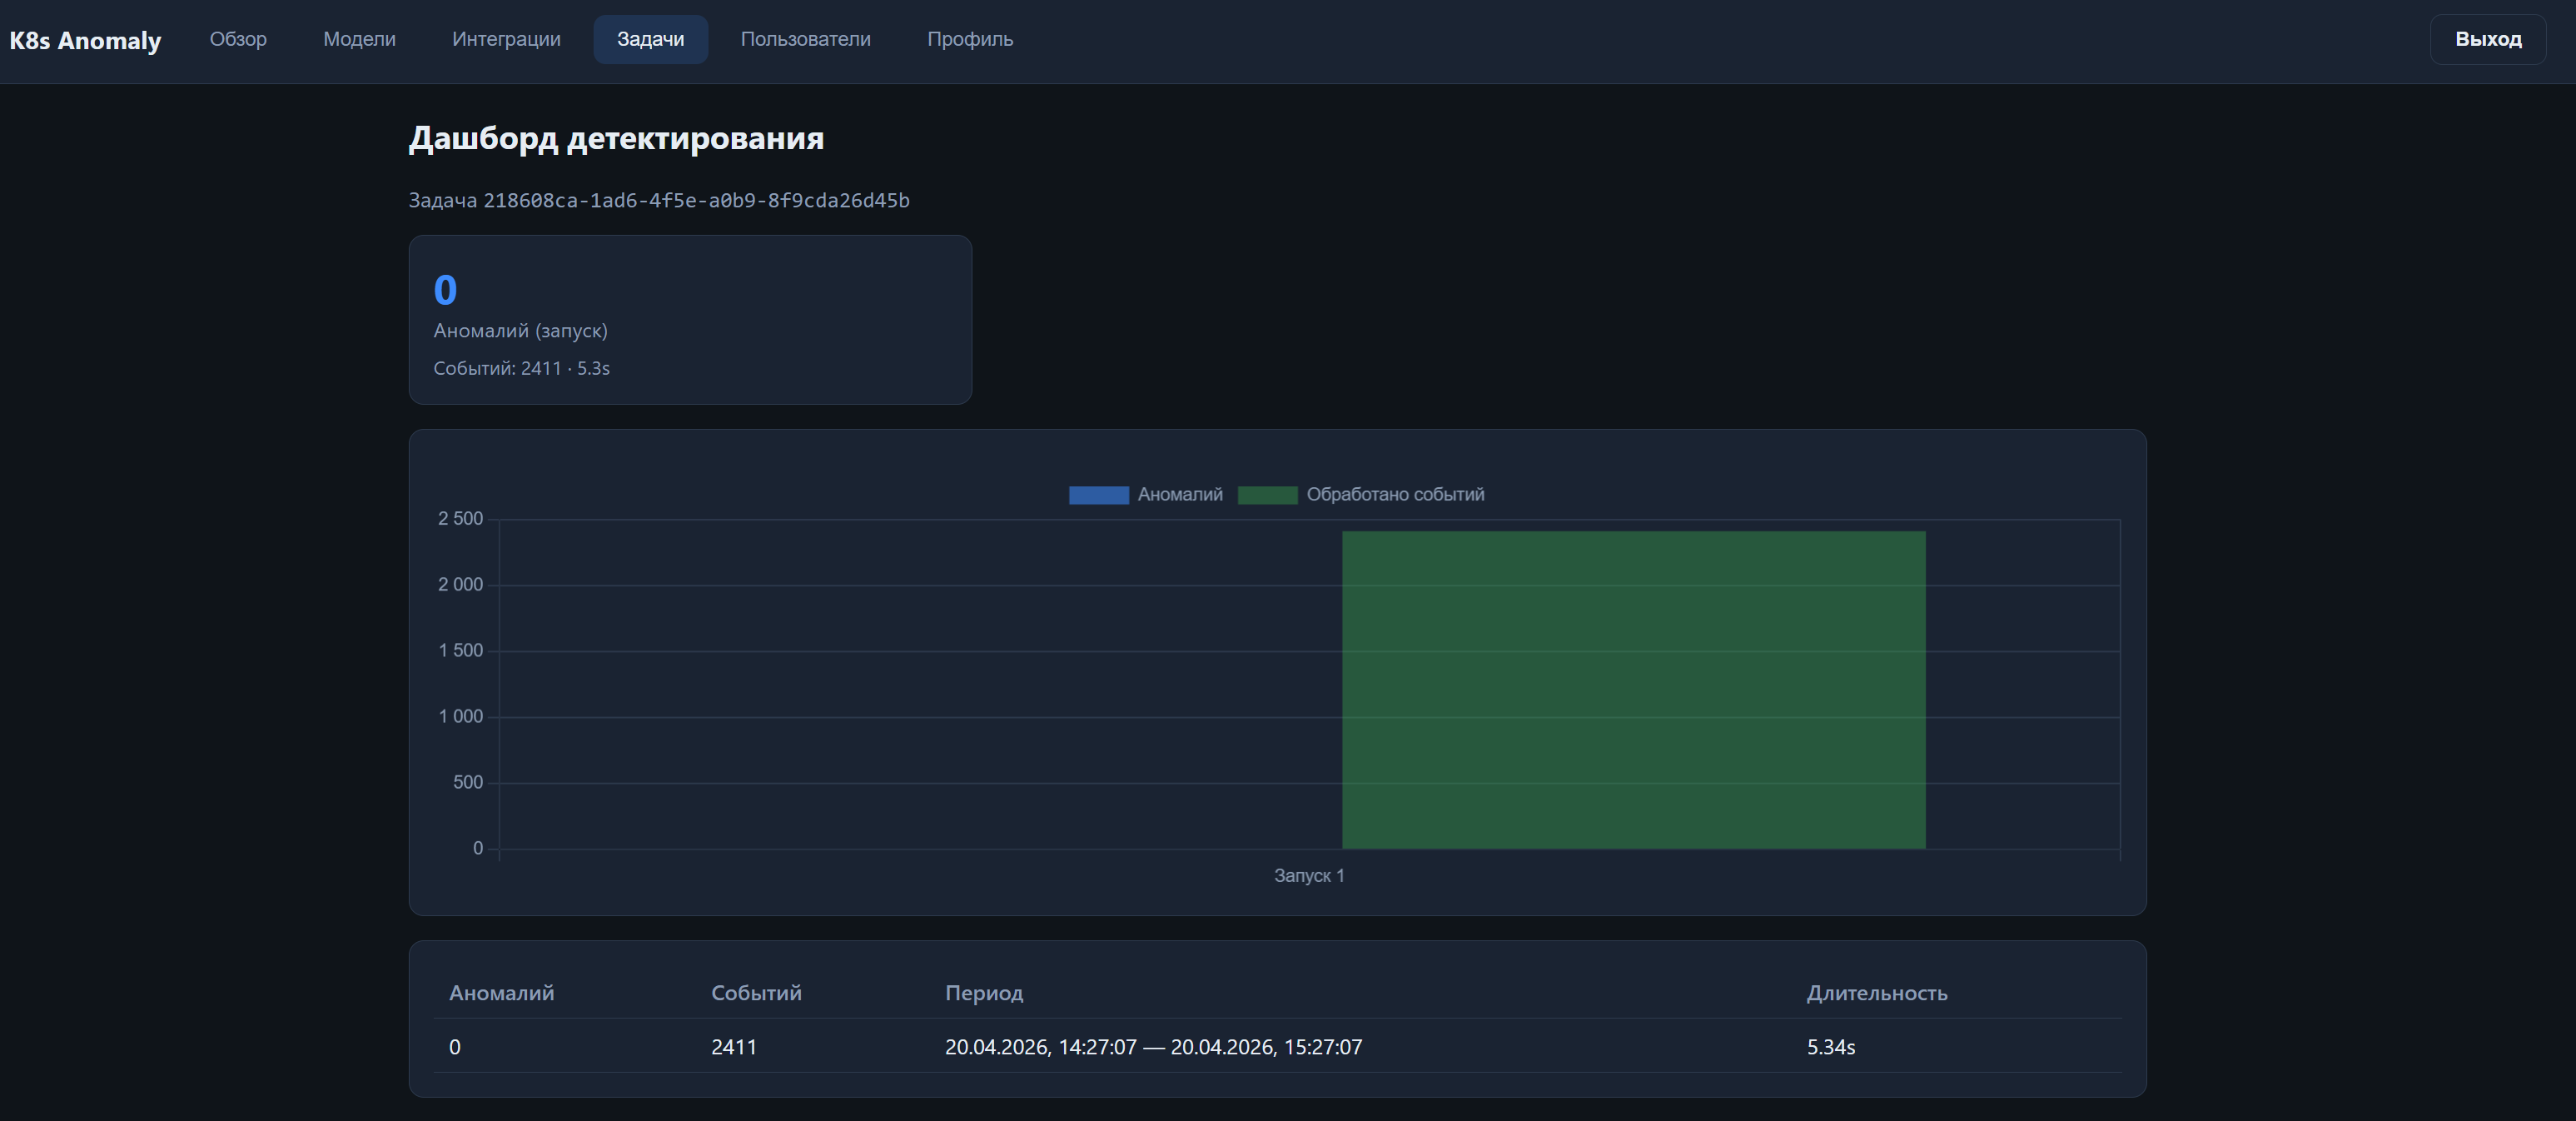
\includegraphics[scale=0.35]{inc/images/metrics_example}
    \caption{Пример метрик выполнения задачи обнаружения аномалий}
    \label{fig:metrics_example}
\end{figure}